% Options for packages loaded elsewhere
\PassOptionsToPackage{unicode}{hyperref}
\PassOptionsToPackage{hyphens}{url}
%
\documentclass[
]{book}
\usepackage{lmodern}
\usepackage{amssymb,amsmath}
\usepackage{ifxetex,ifluatex}
\ifnum 0\ifxetex 1\fi\ifluatex 1\fi=0 % if pdftex
  \usepackage[T1]{fontenc}
  \usepackage[utf8]{inputenc}
  \usepackage{textcomp} % provide euro and other symbols
\else % if luatex or xetex
  \usepackage{unicode-math}
  \defaultfontfeatures{Scale=MatchLowercase}
  \defaultfontfeatures[\rmfamily]{Ligatures=TeX,Scale=1}
\fi
% Use upquote if available, for straight quotes in verbatim environments
\IfFileExists{upquote.sty}{\usepackage{upquote}}{}
\IfFileExists{microtype.sty}{% use microtype if available
  \usepackage[]{microtype}
  \UseMicrotypeSet[protrusion]{basicmath} % disable protrusion for tt fonts
}{}
\makeatletter
\@ifundefined{KOMAClassName}{% if non-KOMA class
  \IfFileExists{parskip.sty}{%
    \usepackage{parskip}
  }{% else
    \setlength{\parindent}{0pt}
    \setlength{\parskip}{6pt plus 2pt minus 1pt}}
}{% if KOMA class
  \KOMAoptions{parskip=half}}
\makeatother
\usepackage{xcolor}
\IfFileExists{xurl.sty}{\usepackage{xurl}}{} % add URL line breaks if available
\IfFileExists{bookmark.sty}{\usepackage{bookmark}}{\usepackage{hyperref}}
\hypersetup{
  pdftitle={Social Isolation},
  pdfauthor={Livia Tomova, Sarah-Jayne Blakemore, Emily Towner},
  hidelinks,
  pdfcreator={LaTeX via pandoc}}
\urlstyle{same} % disable monospaced font for URLs
\usepackage{longtable,booktabs}
% Correct order of tables after \paragraph or \subparagraph
\usepackage{etoolbox}
\makeatletter
\patchcmd\longtable{\par}{\if@noskipsec\mbox{}\fi\par}{}{}
\makeatother
% Allow footnotes in longtable head/foot
\IfFileExists{footnotehyper.sty}{\usepackage{footnotehyper}}{\usepackage{footnote}}
\makesavenoteenv{longtable}
\usepackage{graphicx}
\makeatletter
\def\maxwidth{\ifdim\Gin@nat@width>\linewidth\linewidth\else\Gin@nat@width\fi}
\def\maxheight{\ifdim\Gin@nat@height>\textheight\textheight\else\Gin@nat@height\fi}
\makeatother
% Scale images if necessary, so that they will not overflow the page
% margins by default, and it is still possible to overwrite the defaults
% using explicit options in \includegraphics[width, height, ...]{}
\setkeys{Gin}{width=\maxwidth,height=\maxheight,keepaspectratio}
% Set default figure placement to htbp
\makeatletter
\def\fps@figure{htbp}
\makeatother
\setlength{\emergencystretch}{3em} % prevent overfull lines
\providecommand{\tightlist}{%
  \setlength{\itemsep}{0pt}\setlength{\parskip}{0pt}}
\setcounter{secnumdepth}{5}
\usepackage{booktabs}
\usepackage[]{natbib}
\bibliographystyle{apalike}

\title{Social Isolation}
\author{Livia Tomova, Sarah-Jayne Blakemore, Emily Towner}
\date{Last updated - 2020-12-17}

\begin{document}
\maketitle

{
\setcounter{tocdepth}{1}
\tableofcontents
}
\hypertarget{social-isolation-study}{%
\chapter{Social Isolation Study}\label{social-isolation-study}}

\hypertarget{intro}{%
\chapter{Introduction}\label{intro}}

\hypertarget{scan-protocol}{%
\chapter{Scan Protocol - 7T}\label{scan-protocol}}

\hypertarget{pre-scan}{%
\section{Pre-Scan}\label{pre-scan}}

\hypertarget{asap}{%
\subsection{ASAP}\label{asap}}

\begin{itemize}
\tightlist
\item
  Send participant COVID risk form
\item
  Send participant information sheet
\item
  Send participant consent/assent forms
\item
  Call participant for MRI safety screening (WBIC form)
\item
  Schedule tentative date for scan
\end{itemize}

\hypertarget{week-prior}{%
\subsection{1 Week Prior}\label{week-prior}}

\begin{itemize}
\tightlist
\item
  Send WBIC the completed COVID risk form
\item
  Send WBIC the completed MRI safety screening (WBIC form)
\item
  Book scan session with WBIC (\href{mailto:bookings@wbic.acm.ac.uk}{\nolinkurl{bookings@wbic.acm.ac.uk}})
\item
  Schedule participant COVID safety screening call (must be 48 hrs prior to scan)
\end{itemize}

\hypertarget{hours-prior}{%
\subsection{48 Hours Prior}\label{hours-prior}}

\begin{itemize}
\tightlist
\item
  Call participant for COVID safety screening
\item
  Make sure Teams App on phone and shift assigned for WBIC
\end{itemize}

\hypertarget{night-before}{%
\subsection{Night Before}\label{night-before}}

\begin{itemize}
\tightlist
\item
  Charge laptop
\item
  Plan to arrive 20 minutes early
\item
  Email participant reminder to arrive 15 minutes early
\end{itemize}

\hypertarget{scan}{%
\section{Scan}\label{scan}}

\hypertarget{on-arrival}{%
\subsection{On Arrival}\label{on-arrival}}

\begin{itemize}
\tightlist
\item
  Send message in teams COVID-19 channel ``I'm here''
\item
  Tell receptionist you are scanning on 7T with your assigned Radiographer (Tracy)
\item
  Find place in lobby to sit
\item
  Have participant fill out MRI safety screening (again)
\item
  Load task on laptop (disinfect laptop - COVID protocol)

  \begin{itemize}
  \tightlist
  \item
    Password - frith3
  \item
    \protect\hyperlink{disabling-wifi-on-windows}{Disabling WiFi on Windows}
  \item
    Close all applications
  \end{itemize}
\item
  Run practice task (approximately 5 minutes duration)

  \begin{itemize}
  \tightlist
  \item
    Open MatLab
  \item
    Set current directory as task directory
  \item
    Type MID\_v9 and hit ``Enter''
  \item
    Type participant id - pilot\_02
  \item
    Type ``0'' to run practice
  \end{itemize}
\end{itemize}

\hypertarget{practice-task-instructions}{%
\subsection{Practice Task Instructions}\label{practice-task-instructions}}

\begin{itemize}
\tightlist
\item
  Explain task
\end{itemize}

\begin{quote}
In this task, you are playing for real money! Your goal is to make as much money as possible! Each trial will begin with a cross. You will then see a star with a number inside. The number inside the star indicates how much money you can earn or lose on each trial. After each star you will see a white circle - followed by a white square. Your job is to respond to the white square by pressing the button as quickly as possible.
\end{quote}

\begin{quote}
If you press the button quick enough on a win trial, you will win the amount in the star. If you press the button quick enough on a lose trial, you will avoid losing the amount in the star. Your earnings and losses will add up and you are playing for real money - so be sure to pay close attention and press the button as quickly as you can when you see the white square.
\end{quote}

\begin{itemize}
\tightlist
\item
  Have participant explain task back to you
\end{itemize}

\hypertarget{scan-setup}{%
\subsection{Scan Setup}\label{scan-setup}}

\begin{itemize}
\tightlist
\item
  Radiographer will assist participant into scanner

  \begin{itemize}
  \tightlist
  \item
    Explain emergency squeeze ball, hearing protection, talking between each run
  \item
    Explain staying VERY STILL - even small movements will cause distortions
  \item
    Using button box to respond to task (press \#1)
  \end{itemize}
\item
  Connect laptop

  \begin{itemize}
  \tightlist
  \item
    To projector
  \item
    To trigger
  \item
    Plug in to power outlet
  \end{itemize}
\item
  Setup task (should be setup from practice run)
\item
  If Cat not present, tell radiographer to cut one DTI sequence (keep the MB2\_iPAT2)
\end{itemize}

\hypertarget{scanning}{%
\subsection{Scanning}\label{scanning}}

\begin{itemize}
\tightlist
\item
  Scan sequences are saved in protocol at WBIC
\item
  Radiographer or researcher to check in with participant after each run
\item
  Anatomical scans first
\item
  Functional scans

  \begin{itemize}
  \tightlist
  \item
    Type MID\_v9 and hit ``Enter''
  \item
    Type participant id - pilot\_02
  \item
    Type ``1'' to run first run
  \item
    When complete run other 3 runs (\#2-4)
  \end{itemize}
\end{itemize}

\hypertarget{post-scan}{%
\section{Post Scan}\label{post-scan}}

\begin{itemize}
\tightlist
\item
  Ask pilot participant (make notes)

  \begin{itemize}
  \tightlist
  \item
    Was there anything they did not understand?
  \item
    Was there anything strange or different than expected?
  \item
    How were the timings? Were they fast, but long enough to understand?
  \end{itemize}
\end{itemize}

\hypertarget{on-exit}{%
\subsection{On Exit}\label{on-exit}}

\begin{itemize}
\tightlist
\item
  Send message in teams COVID-19 channel ``I'm leaving''
\item
  Backup behavioral data
\item
  Livia to download scan data from cluster
\end{itemize}

\begin{center}\rule{0.5\linewidth}{0.5pt}\end{center}

\hypertarget{troubleshooting}{%
\section{Troubleshooting}\label{troubleshooting}}

For help/advice please do not hesitate to contact the WBIC Radiographers \href{mailto:wbic-radiog@lists.cam.ac.uk}{\nolinkurl{wbic-radiog@lists.cam.ac.uk}}.

\hypertarget{disabling-wifi-on-windows}{%
\subsection{Disabling WiFi on Windows}\label{disabling-wifi-on-windows}}

\begin{enumerate}
\def\labelenumi{\arabic{enumi}.}
\tightlist
\item
  Go to the Start Menu and select Control Panel
\item
  Click the Network And Internet category\\
  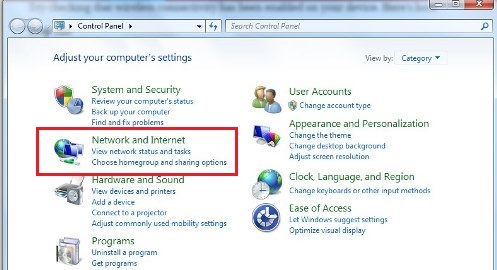
\includegraphics{images/scan_protocol/1.jpg}
\item
  Select Networking and Sharing Center\\
  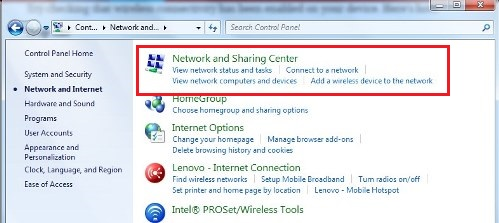
\includegraphics{images/scan_protocol/2.jpg}
\item
  From the options on the left-hand side, select Change adapter settings\\
  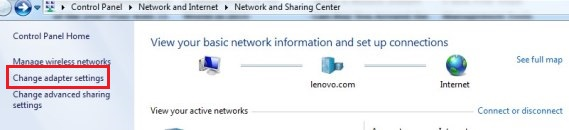
\includegraphics{images/scan_protocol/3.jpg}
\item
  Right click on Wireless Network Connection\\
  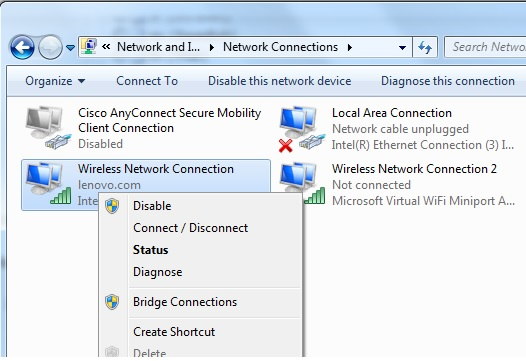
\includegraphics{images/scan_protocol/4.jpg}
\item
  Select ``Disable''
\end{enumerate}

\hypertarget{finding-the-wbic}{%
\subsection{Finding the WBIC}\label{finding-the-wbic}}

\begin{itemize}
\tightlist
\item
  Google WBIC and follow maps
\item
  There will be a roundabout near the hospital
\item
  Entrance to WBIC is at end of the street past the hospital
\end{itemize}

  \bibliography{references.bib,packages.bib}

\end{document}
